\chapter{Design And Implementation}

\section{Overall Design}
\par
NetDog follows the client-server architecture. What this means is that, NetDog
has both a client part and a server part. The server part is meant to be run
on the machine used by the system administrator, while the client part runs
on the rest of the machines on the network.\\

Both the server and client listens for connections from each other, allowing
the server to execute commands on clients and the client to report back any
progress. But the server has an additional capability that the clients lack, an
easy to use web interface that can be used by the administrator to control the
machines and configure the server.

\section{User Interfaces}
NetDog is a very easy to use system. One of the main aims while designing the
system was to abstract as much lower level details of the system as possible
from the user. There is no user interface for the client machines. All of the
system is controlled from the server. The server provides a command line
interface and a very convinient web interface for administration. The whole
system can be operated and configured from these interfaces.

\section{Hardware Interfaces}
The system tries hard not to reinvent the wheel. Thus, it uses existing Linux
subsystems as much as possible. As a side effect, NetDog can work with any
networking hardware supported by Linux. If the clients on the network can
succesfully communicate over the network using their network interface cards,
you are good to go.

\section{Communications Interfaces}
The system uses the TCP/IP system for communication between server and clients.
On top of TCP, the system uses a home grown higher level "NetDog" protocol for
coordinating the client machine and servers. It is the NetDog protocol that
ensures efficient communication and security. The protocol specification is
under heavy development and the exact specification will be relased in further
revisions of this document.

\section{System Design}
\par
On a lower level, the design of NetDog is a bit different. NetDog is splitted
into three modules, the server module, the client module and the web server
module. The three of them has distinct functions. But the interesting fact is,
both the client module and the server module share the same underpinnings. All
the functions they use are from a library called libgreen, that was built
specifically for use in NetDog.

% debug: include image

\subsection{NetDog Server}
\par
The NetDog server module acts as the server. The server module resides in the
file ``netdog\_server.py'' It uses functions part of the libgreen library to
setup a server working on the netdog protocol.\\

It listens for connections from clients on port 1337 and also provides the web
interface. The server is completeley multithreaded and this allows it to
perform tasks involving hundreds of machines at a surprisingly quick rate.

\subsection{NetDog client}
\par
The NetDog client module is the part of NetDog that is run on the client
machines. The client module listens for connections from the server at port
1994. Once a connection is received, it is handled as per the command it
contains.

\subsection{Web Server}
\par
The webserver module provides the web interface for use by the administrator.
Written using the bottle library, it resides in the file ``web\_server.py''. The
web server also uses the libgreen library extensively, to serve its clients. It
is not directly invoked from the file, rather the contents of ``web\_server.py''
is imported into ``netdog\_server.py'' and started as a separate thread.

\subsection{NetDog protocol}
\par
The NetDog client and server operates using the NetDog protocol. NetDog protocol
is a custom built protocol, that has been developed on top of the Sockets
library part of standard Python installation. The mechanism as well as the
policies for the protocol is defined inside the libgreen library.\\

The NetDog protocol defines the structure of messages passed between the server
and the clients. The message has primarily three parts:

\begin{itemize}
    \item Hostname, which is the hostname of the sender
    \item encrypted flag, whether the message is encrypted or not
    \item data, which is further divided into command and payload
\end{itemize}

\begin{figure}[H]
\centering
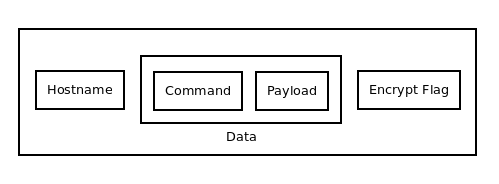
\includegraphics[scale=0.6]{protocol}
\caption{NetDog protocol message structure}
\end{figure}

\subsection{DataFlow Diagram}
A data flow diagram (DFD) is a graphical representation of the "flow" of data
through an information system, modelling its process aspects. A DFD is often
used as a preliminary step to create an overview of the system without going
into great detail, which can later be elaborated. DFDs can also be used for the
visualization of data processing (structured design).\\

A DFD shows what kind of information will be input to and output from the
system, how the data will advance through the system, and where the data will
be stored. It does not show information about process timing or whether
processes will operate in sequence or in parallel, unlike a traditional
structured flowchart which focuses on control flow, or a UML activity workflow
diagram, which presents both control and data flows as a unified model.

\begin{figure}[H]
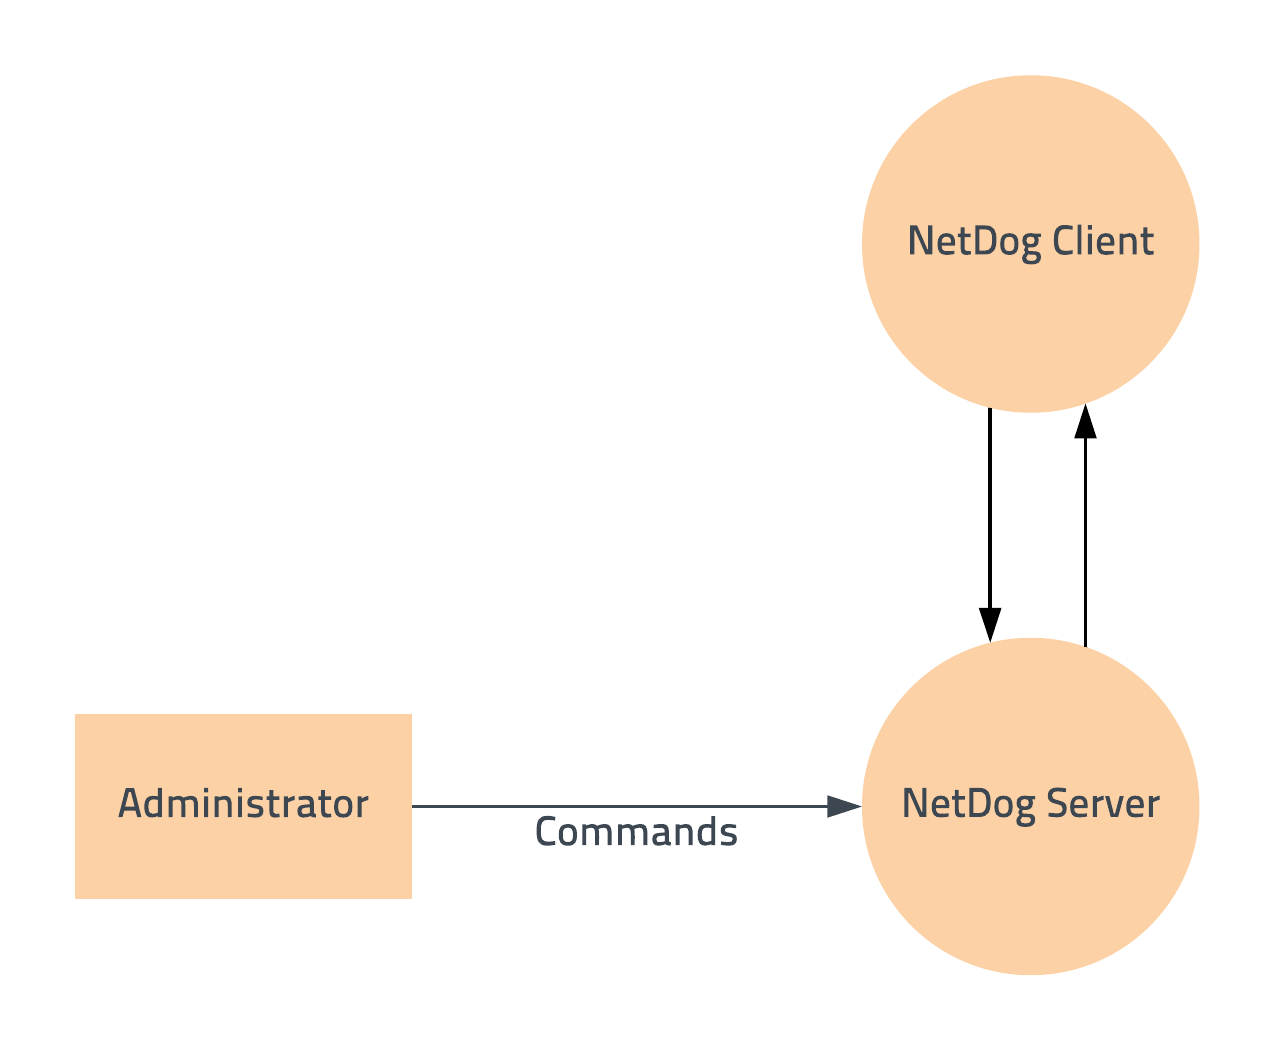
\includegraphics{dfd_level_0}
\caption{Level 0 Data Flow}
\end{figure}

\begin{figure}[H]
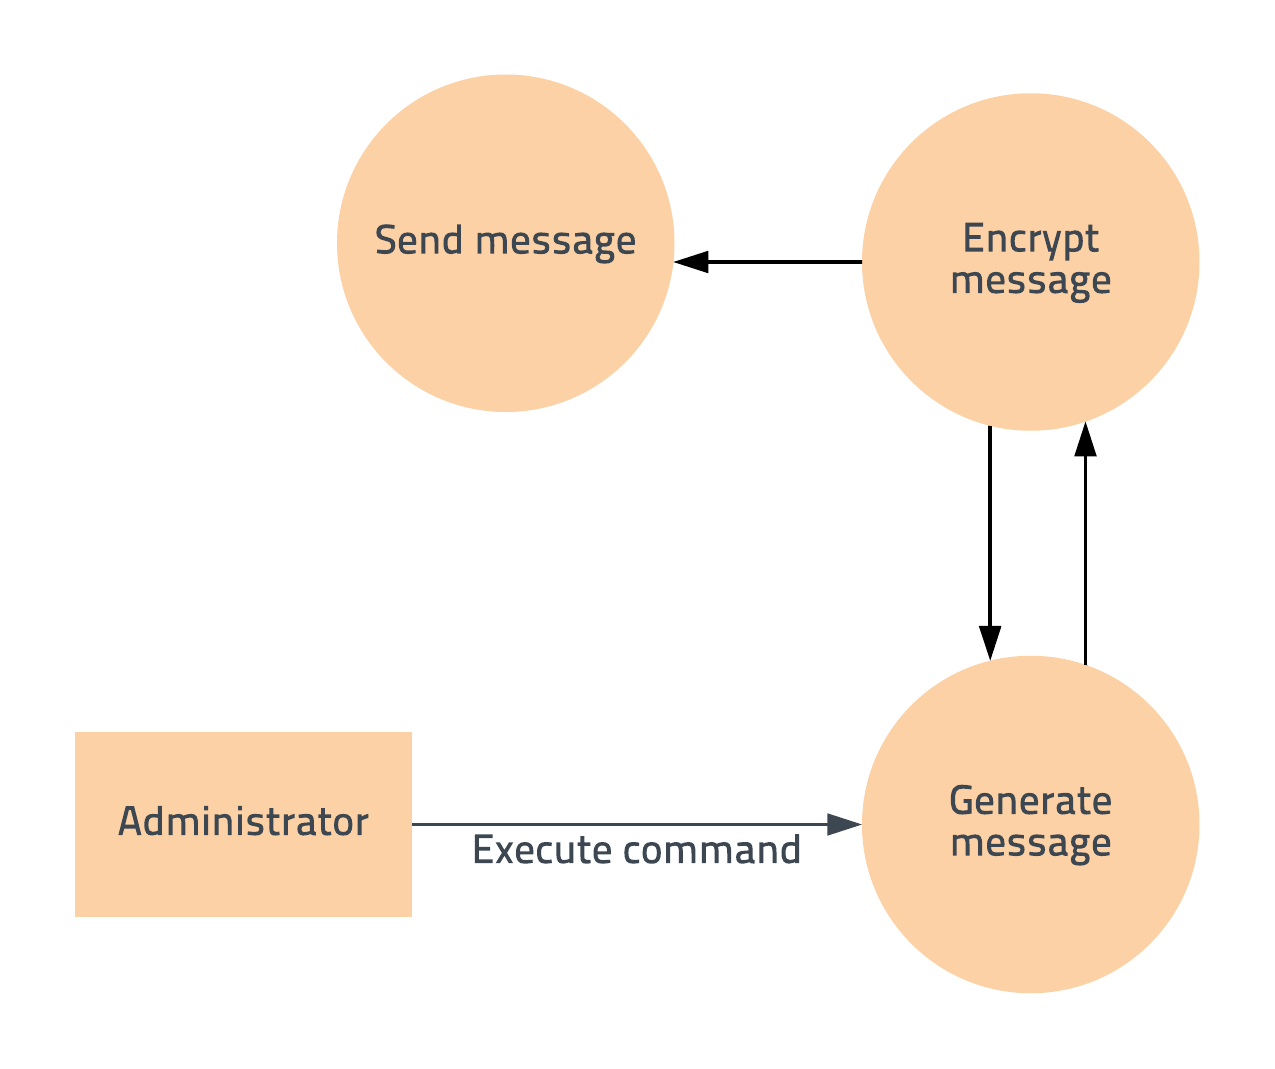
\includegraphics{dfd_level_1}
\caption{Level 1 Data Flow}
\end{figure}

\subsection{Screenshots}

\begin{figure}[H]
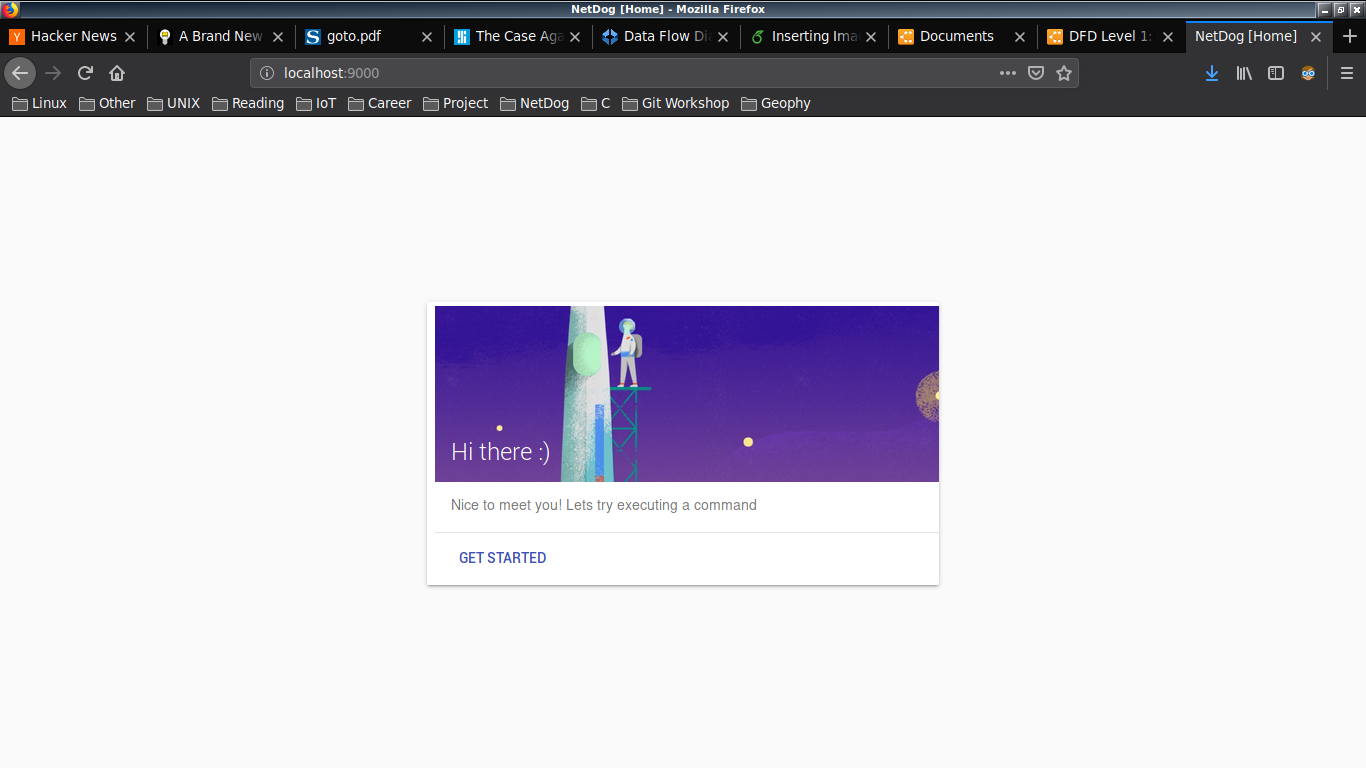
\includegraphics[scale=0.3]{netdog_home}
\caption{NetDog Home Page}
\end{figure}

\begin{figure}[H]
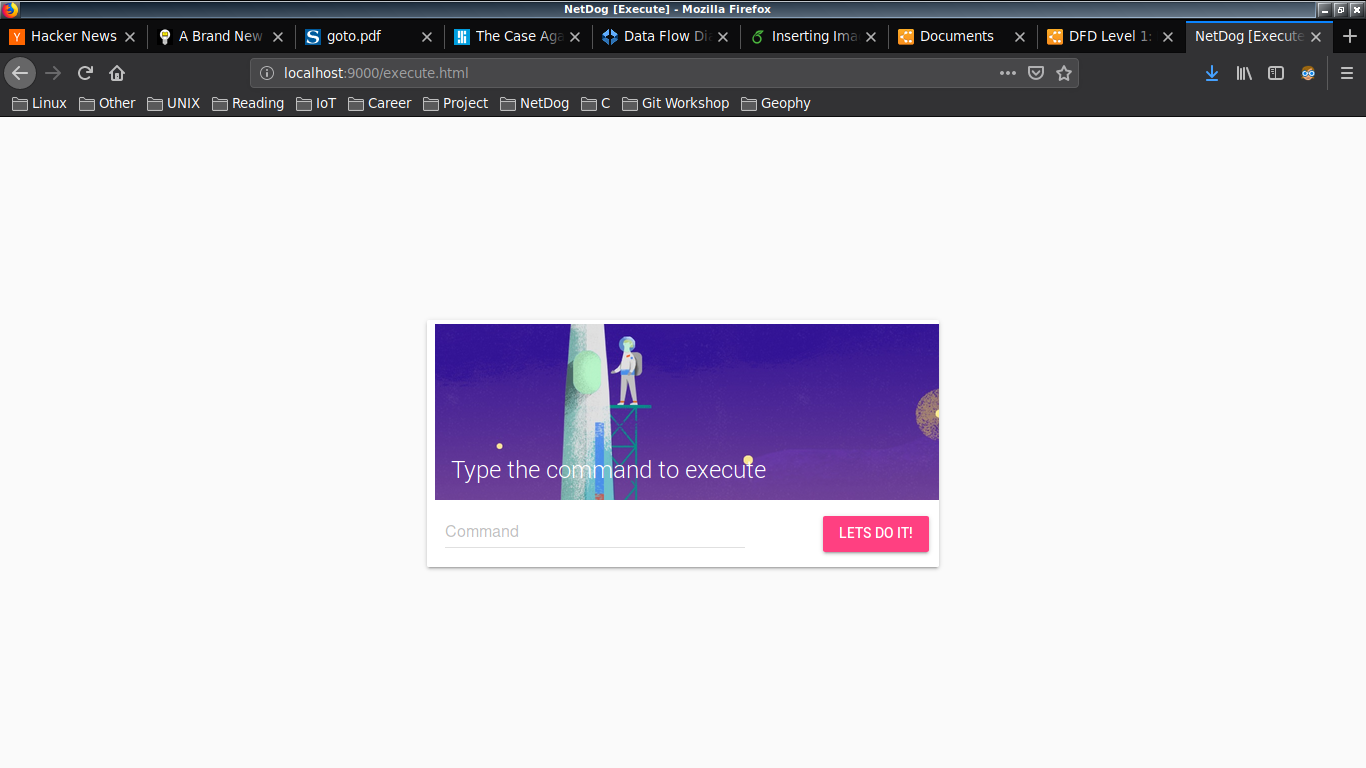
\includegraphics[scale=0.3]{netdog_execute}
\caption{NetDog Execute command page}
\end{figure}

\begin{figure}[H]
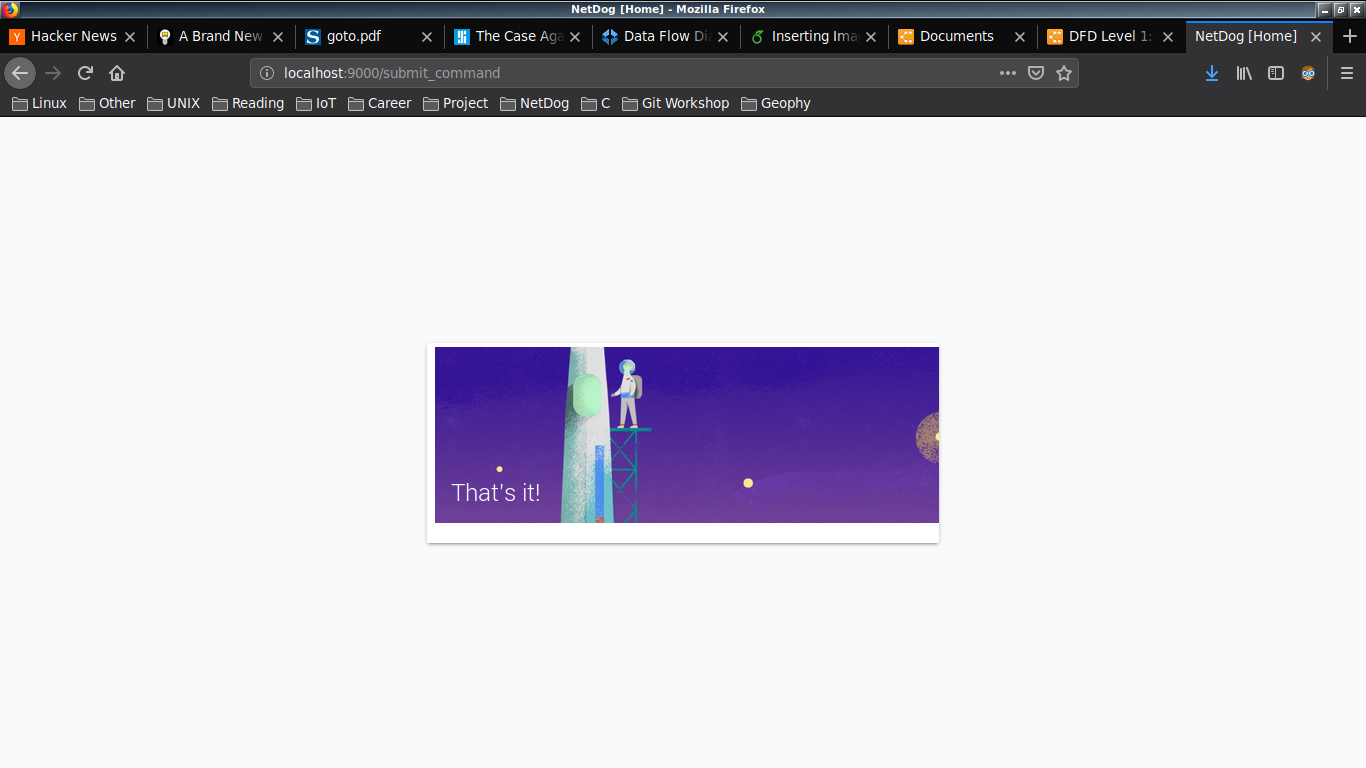
\includegraphics[scale=0.3]{netdog_success}
\caption{NetDog success page}
\end{figure}

